\newpage
\subsection{Caso d'uso UC15: Login con Twitter}
\label{UC15}
\begin{figure}
	\centering
	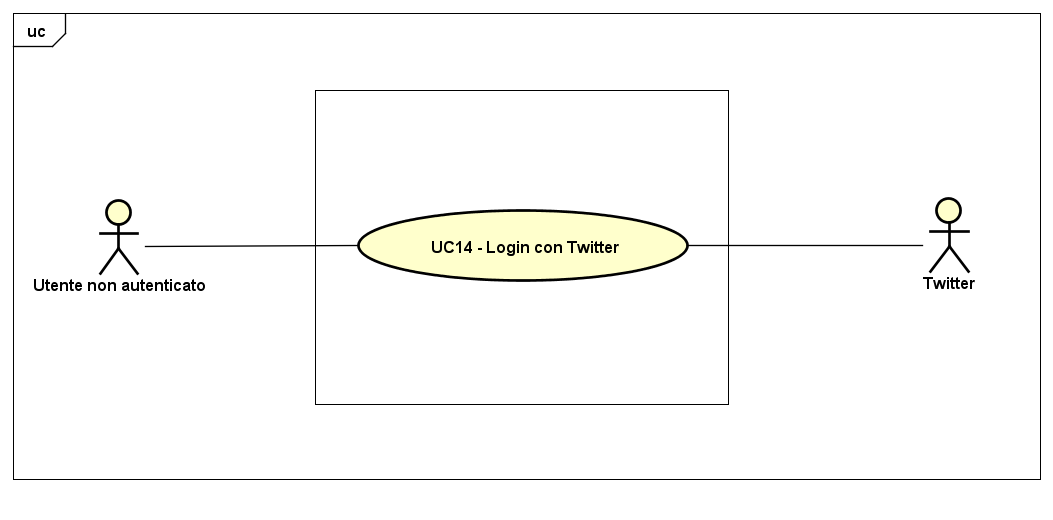
\includegraphics[scale=0.48]{UML/UC15.png}
	\caption{UC15: Login da Twitter}
\end{figure}
\FloatBarrier
\begin{itemize}
	\item \textbf{Attori}: utente non autenticato, Twitter;
	\item \textbf{Scopo e descrizione}: l'attore può autenticarsi utilizzando Twitter;
	\item \textbf{Precondizione}: l'attore visualizza la pagina di login e sceglie il login con Twitter;
	\item \textbf{Postcondizione}: l'attore è autenticato;
	\item \textbf{Scenario principale}: l'attore effettua il login tramite Twitter.
\end{itemize}
